\documentclass[10pt,a4paper]{article}
\usepackage[margin=1in]{geometry}
\usepackage{amsmath,amsthm,amssymb}
\usepackage{amsfonts}
\usepackage{relsize}
\usepackage{graphicx}
\usepackage{float}
\usepackage{subcaption}
\graphicspath{ {Bayesian_Project/} }
\usepackage{listings}
\usepackage{color}
\definecolor{light-gray}{gray}{0.92}
\usepackage{fancyhdr}
\pagestyle{fancy}
\usepackage{sectsty}
 
\sectionfont{\fontsize{15}{18}\selectfont}

\begin{document}
\title{\vspace{-3cm} \textsc{\normalsize EN.553.732  Project Report}\\ \text{} \\ \textsc{\large A Prediction of MLB Batting Averages: \\ A Comparison Between Bayesian and Frequentist Approaches}}
\author{\textsc{\normalsize Joseph High, Kenneth Feder \& Joseph Yu}}
\date{\small December 22, 2017}
\maketitle

\section*{\large Purpose} 
The goal of our project is to determine whether a Bayesian approach or a frequentist approach would prove to be more suitable in predicting a professional baseball player's future batting average, a traditional measure of player performance. 
\section*{\large Motivation and Background} 
Forecasting future performance in Major League Baseball is an ongoing area of interest in the statistical community and, of course, in the baseball community. There is no shortage of literature on the subject and data collection has been made very convenient as public databases are regularly updated by those in the baseball community. In fact, there is an entire academic field dedicated to collecting and analyzing baseball statistics. Sabermetrics makes use of many areas of mathematics in order to answer several types of questions that arise in baseball, but statistics is the main tool of a sabermetrician. One of the primary goals of a sabermetrician is to predict player performance and to improve and find new measures of player performance. A traditional measure of a player's performance is his batting average, which is simply the player's total number of hits divided by his total number of at-bats. \par 
Predicting player performance became a particular area of interest in the 2002 season when the Oakland Athletics, who at that time had the third lowest payroll in the MLB, made it to the playoffs by leveraging Sabermetric principles.
\section*{\large Data}
Our data was acquired from Lahman's Baseball Database (http://www.seanlahman.com/baseball-archive/
statistics/). The data is seasonal and extensive, covering player statistics from the 1871 season up to the 2016 season. For example, the database includes every professional baseball player's weight, height, and age at the beginning of each season, whether they bat right- or left-handed, each player's seasonal batting statistics, their defensive position, salary, etc. \par
We found it necessary to impose constraints on the data being used. In particular, only data after the 1901 season was used since before this time the American League, who play by a slightly different set of rules, did not exist. Second we limited the data to players that had at least 100 at-bats per season. The reason for this was (Kenny, would you mind filling this in?). Third, only players who played in either the National League or the American League were included since between 1901 and 2016 there did exist other leagues in Major League Baseball who were governed by a different set of rules, rules that would ultimately decrease the reliability of our model (Feel free to edit this as well).
\section*{\large Literature Review}  
!!--This is a required section, but we didn't really review any literature. Refer to note.--!!

\section*{\large Methodology}
We used a hierarchical linear regression model to model our data and fit the model using both a frequentist approach and a Bayesian approach and compared the results. In particular, an EM algorithm was used to fit the frequentist model and used Gibbs sampling facilitate fitting the Bayesian model.  \\
\\\
\textbf{\small Frequentist Model}\\
The outcome of interest is each player's batting average, $B_{ij}$, where each player is indexed by $i$ and each season by $j$, and so $B_{ij}$ represents the seasonal batting average of player $i$ in season $j$. Specifically, we modeled each player's batting average, $B_{ij}$, where for each $i$ and $j$ we let $B_{ij} \sim$ Normal$\mathlarger{\left(\mu_{ij}, \frac{1}{\tau_{avg}}\right)}$ \\
\\\
Our predictor variables relating to a player's performance were his seasonal batting averages in the 2 most recent seasons, $B_{i, j-1}$ and $B_{i, j-2}$. Because a player's performance tends to decrease with age, we used player age as a non-performance predictor variable: \texttt{age}$_{ij}$. It is expected that age have a nonlinear affect on a player's batting average; more precisely, we expect age to have a quadratic affect on a player's batting performance. Thus, our mean within-group model of player $i$'s batting average in season $j$ is $$\mu_{ij} = \beta_{0i} + \beta_1B_{i, j-1} + \beta_2B_{i, j-2} + \beta_3\textrm{\texttt{age}}_{ij} + \beta_4\textrm{\texttt{age}}_{ij}^2$$
Observe that we have allowed the intercept term to vary. That is, for each player $i$, we assign a unique intercept term $\beta_{0i}$. Meanwhile, the $\beta_k, k = 1,...,4$, remain fixed across "groups". Thus, we do indeed have a hierarchical mixed-effects model. \\
Then, for each $i$ we let $\beta_{0i} \sim$ Normal$\mathlarger{\left(\theta_i, \frac{1}{\tau_{_{\beta0}}}\right)}$ where $\theta_i$ can be thought of as each player's career mean. We then modeled $\theta_i$, for each $i$, such that $$\theta_i = \gamma_0 + \gamma_1\textrm{\texttt{height}}_{i} + \gamma_2\textrm{\texttt{height}}_{i}^2 + \gamma_3\textrm{\texttt{weight}}_{i} + \gamma_4\textrm{\texttt{weight}}_{i}^2 + \gamma_5\textrm{\texttt{year}}_{i} + $$ $$ \ \ \ \ \ \ \ \ \ \ \ \ \ \ \ \ \ \ \ \ \ \ \ \ + \ \gamma_6\textrm{\texttt{era}}_{liveball} + \gamma_7\textrm{\texttt{era}}_{expansion} + \gamma_8\textrm{\texttt{era}}_{freeagency} + \gamma_9\textrm{\texttt{era}}_{steroid} + \gamma_{10}\textrm{\texttt{era}}_{modern}$$
where \ \texttt{height}, \texttt{weight} and \texttt{year} represent a player's height, a player's weight, and the year corresponding to season $j$ in the overall within-group model, respectively. In addition, the \texttt{era}$_t$ covariates represent all of the different eras of Major League Baseball, where we have allowed each corresponding $\gamma_t$ time slope to change within each era. We thought it necessary to incorporate this into our model considering the era a player played in could potentially have a significant effect on his batting average. For instance, the steroid era represents a time when a majority of players were using performance enhancing drugs, implying a significant improvement in batting averages, so including this information is meaningful to our model.\\
\\\
\textbf{\small Bayesian Model}\\
For a reliable comparison, we used a hierarchical linear regression model for our Bayesian model as well. However, for the Bayesian model, each of the parameters in both the within-group model and the between-group model were assigned non-informative normal priors and the precisions on the Gaussian distributions were assigned Gamma priors. In particular, we let \\ $$\hspace{-1cm}\beta_k \sim \textrm{Normal(0, 1000)} \ , \ \ k = 1,..., 4   \hspace{2cm}\gamma_s \sim \textrm{Normal(0, 1000)} \ , \ \ s = 1,..., 10$$ $$\hspace{-2.9cm} \ \ \tau_{avg} \sim \textrm{Gamma(0.001, 0.001)} \ \ \ \ \ \ \ \ \ \  \hspace{2.1cm}\tau_{\beta0} \sim \textrm{Gamma(0.001, 0.001)}$$
To obtain our model parameters, we used a Bayesian computational engine called JAGS (Just Another Gibbs Sampler) which is designed specifically for the analysis of Bayesian hierarchical models. It allows the user to specify the priors in advance and facilitates the analysis of the model using Gibbs sampling.

\section*{\large Data Analysis and Interpretation}
We begin by examining the data to get an idea of what we are working with. A plot of the empirical distribution of the data was developed and can be seen below in Figure 1(a). To be more specific, Figure 1(a) is a histogram of all batting averages from 1901 to present which satisfy the inclusion constraints imposed on our data. It is seen that the histogram is nearly bell-shaped, implying that the Normal distribution is an appropriate choice for our data. We also plot the trajectory of every single professional baseball player, fitting the criteria, from 1901 to present. Each individual continuously connected line, is the career trajectory for one player. Looking at Figure 1(b) more closely we see that there is a secular trend among most of the trajectories. That is, each trajectory tends to remain moving on a similar path throughout it's lifetime. What this says is that players that hit well, tend to hit well, or having higher batting averages, throughout their career while players that hit poorly, tend to have lower batting averages throughout their career. This validates our choice of prior batting averages being used as a predictor for future performance.

\begin{figure}[H]
 
\begin{subfigure}{0.5\textwidth}
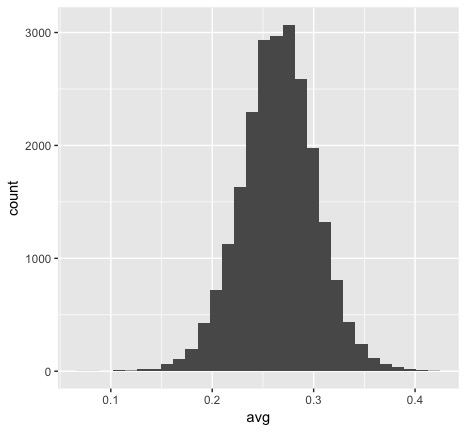
\includegraphics[width=7.5cm,height=7.5cm]{../DataVisHistogram.jpeg} 
\caption{Empirical distribution of the data}
\label{fig:subim1}
\end{subfigure}
\begin{subfigure}{0.5\textwidth}
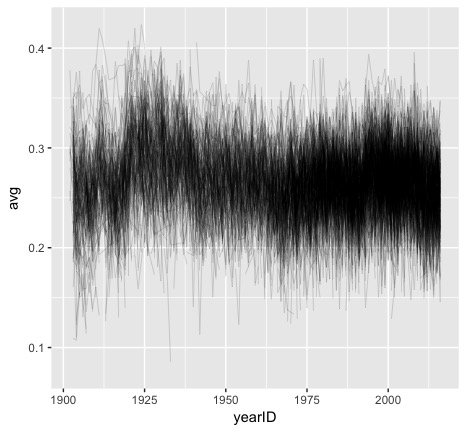
\includegraphics[width=7.5cm,height=7.5cm]{../PastTrajectories.jpeg}
\caption{Player trajectories from 1901 to 2016}
\label{fig:subim2}
\end{subfigure}

\caption{Visualizing and Analyzing the data}
\label{fig:image2}
\end{figure} 

In our first attempt to fit the frequentist model, we see in Figure 2(b) that the data generally has a linear trend to it, but based on the plot alone, we may be able to do better. Referring to Figure 2(a) it can be seen that me might be able to get a better fit if we remove \texttt{height} and it's quadratic term. Indeed, the t-values of \texttt{height} are very close to zero.
\begin{figure}[H]
\begin{subfigure}{0.5\textwidth}
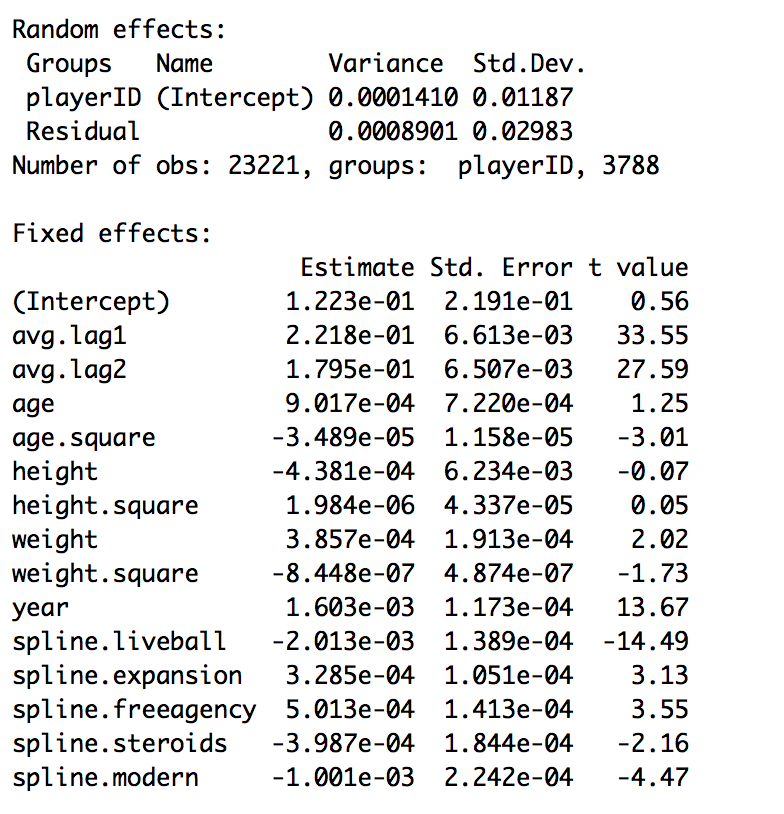
\includegraphics[width=8cm,height=8cm]{../freqsummary}
\caption{Summary from 1st frequentist fit}
\label{fig:subim2}
\end{subfigure}
\begin{subfigure}{0.5\textwidth}
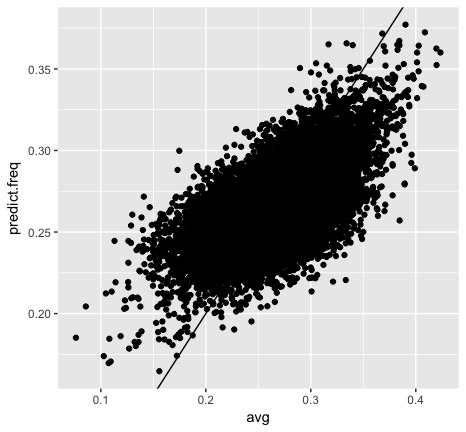
\includegraphics[width=8cm,height=8cm]{../Freqfit_vs_truth.jpeg}
\caption{1st Frequentist Fit}
\label{fig:subim1}
\end{subfigure}

\caption{Predictive Accuracy, 1st Frequentist Fit}
\end{figure}

In our second attempt to fit the frequentist model, it can be seen, in Figure 3, via the t-values of the remaining coefficients that we did indeed do a bit better. However, our prediction plot is extremely similar to that of our first attempt where \texttt{height} is included. This suggests that \texttt{height} has very little predictive power on a player's batting average.
\begin{figure}[H]
\begin{subfigure}{0.5\textwidth}
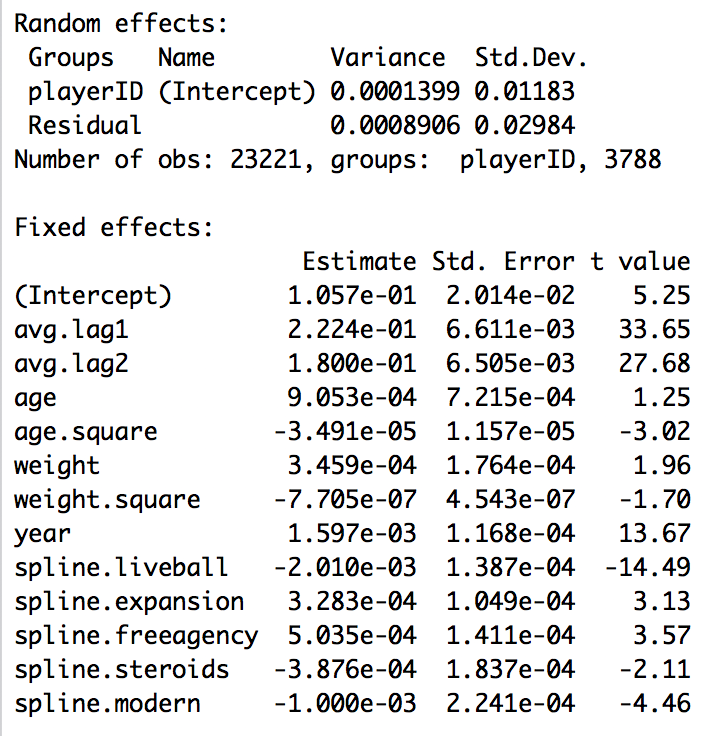
\includegraphics[width=8cm,height=8cm]{../freqsummary2}
\caption{Summary from 1st frequentist fit}
\label{fig:subim2}
\end{subfigure}
\begin{subfigure}{0.5\textwidth}
\includegraphics[width=8cm,height=8cm]{../Freqfit2.jpeg}
\caption{2nd Frequentist Fit}
\label{fig:subim1}
\end{subfigure}

\caption{Predictive Accuracy, 2nd Frequentist Fit}
\end{figure}


\begin{figure}[H]
\begin{center}
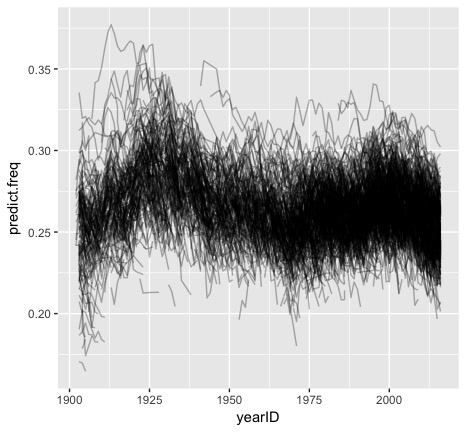
\includegraphics[width=9cm,height=9cm]{../PredictedTrajectories.jpeg}
\caption{}
\label{fig}
\end{center}
\end{figure}

\begin{figure}[H]
\begin{center}
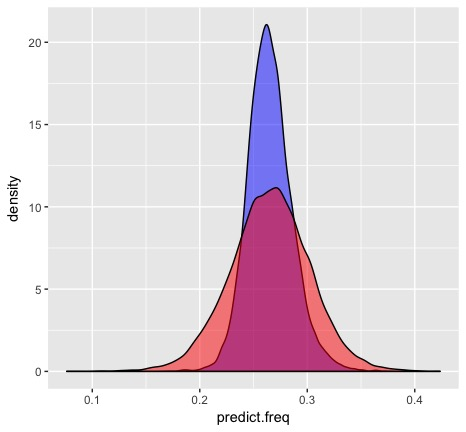
\includegraphics[width=9cm,height=9cm]{../FreqResult.jpeg}
\caption{}
\label{fig}
\end{center}
\end{figure}

\begin{figure}[H]
\begin{center}
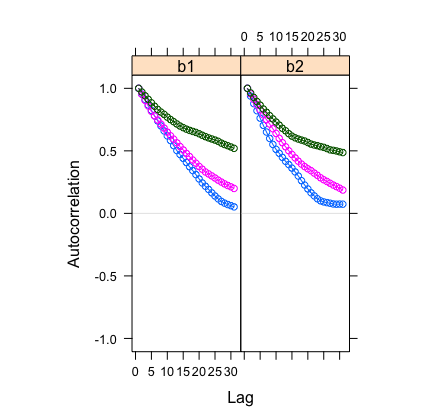
\includegraphics[width=9cm,height=9cm]{../ACFPlot.png}
\caption{}
\label{fig}
\end{center}
\end{figure}

\begin{figure}[H]
\begin{center}
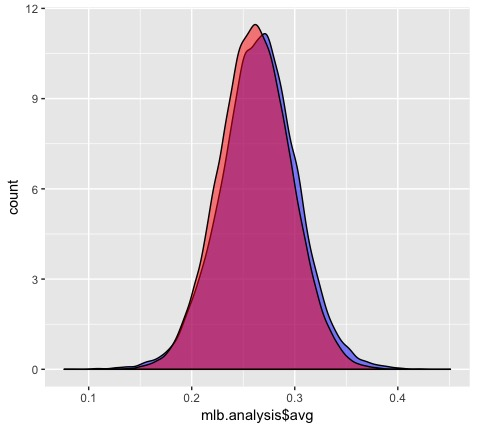
\includegraphics[width=9cm,height=9cm]{../BayesianPredictionPlot.jpeg}
\caption{}
\label{fig1}
\end{center}
\end{figure}

\section*{R Code}
\lstset{backgroundcolor=\color{light-gray}, frame=single, basicstyle = \ttfamily\small}
\begin{lstlisting}{language=R}
# This analysis attempts to predict batting average
# The goal is to compare frequentist and bayesian methods
# Data come from Lahman Baseball data archive, copyright Sean Lahman
# Source: http://www.seanlahman.com/baseball-archive/statistics/
# Authors: Kenneth Feder, Joseph High, Joseph Yu

# Load required packages -- may need to be installed
library(ggplot2)
library(brms)
library(rjags)
library(lme4)
library(plyr)
library(dplyr) 
library(magrittr)
library(coda)
library(beepr)

# Set directory to read in data
setwd("~/Documents/Johns Hopkins/Coursework/Term 9/Bayesian 
           Statistics/Project/baseballdatabank-2017/core") 

# read in player demographics and batting data

master <- read.csv("Master.csv")
batting <- read.csv("Batting.csv")

# Reset directory to working directory
setwd("~/Documents/Johns Hopkins/Coursework/Term 9/Bayesian 
Statistics/Project")

# Merge the two datasets
mlb <- right_join(master,batting,by = "playerID")
summary(mlb)

###################### Preparing for Analysis ######################
head(mlb)
filter(mlb,birthYear == 1852,birthState == "MD")
# Rearrange for easier viewability
mlb %<>% arrange(playerID,yearID)
head(mlb)
summary(mlb)

# Data cleaning for analysis

mlb.analysis <- mlb %>% select(playerID,birthYear,weight,height,
      yearID,teamID,lgID,G,AB,H) %>% # Extract relvant variables...
  filter(yearID > 1900,AB >= 100,lgID == "NL" | lgID == "AL") %>% 
  # Filter only post 1901, at least 100 AB per season, 
  # only NL and AL play
  mutate( # Add transformed variables
    age = yearID - birthYear,
    age.square = age^2,
    year = yearID - 1900,
    spline.liveball = ifelse(yearID < 1920,0,yearID - 1919), 
    # Allow slope to shift at start of liveball era using spline 
    # http://www.netshrine.com/era.html
    spline.expansion = ifelse(yearID < 1961,0,yearID - 1961), 
    # Allow slope to shift at start of expansion era
    spline.freeagency = ifelse(yearID < 1977,0,yearID - 1977), 
    # Allow slope to shift at start of free agency
    spline.steroids = ifelse(yearID < 1994,0,yearID - 1994), 
    # Allow slope to shift at start of steroid era
    spline.modern = ifelse(yearID < 2005,0,yearID - 2004), 
    # Allow slope to shift at start of modern era
    height.square = height^2,
    weight.square = weight^2,
    avg = H/AB
  ) %>% group_by(playerID) %>% # Group by player ID...
  mutate( # So we can create lagged batting average variables 
          # for each player
    avg.lag1 = lag(avg),
    avg.lag2 = lag(avg.lag1),
    season = row_number()
  ) %>% filter(season > 2) %>% # Drop the first two seasons of 
                               # a player's career
  na.omit %>%  # Drop records with missing information (there are a 
# small number of players with no height/weight info from 
# early 1900s)
  as.data.frame()

# Exploratory plot -- histogram of batting averages
plot.raw.dist <- ggplot(mlb.analysis,aes(x = avg)) +
  geom_histogram()
plot.raw.dist

# Exploratory plot -- batting trends over time
plot.raw.trends <- ggplot(mlb.analysis,aes(yearID,avg, 
          group = playerID)) + geom_line(size = .1, alpha = .5) 
plot.raw.trends

################ Fit frequentist multi-level model ################
names(mlb.analysis)
fit.freq <- lmer(avg ~ avg.lag1 + avg.lag2 + age + age.square + 
                   height + height.square + weight + weight.square + 
                   year + spline.liveball + spline.expansion + 
                   spline.freeagency + spline.steroids + 
                   spline.modern + (1|playerID),
                 data = mlb.analysis)
summary(fit.freq)

# Predictive accuracy
mlb.analysis$predict.freq <- predict(fit.freq)
plot.freqfits.vs.truth <- ggplot(mlb.analysis,aes(avg,predict.freq)) 
   + geom_point() + geom_abline(slope = 1,intercept = 0)
plot.freqfits.vs.truth

# A few example trajectories from post 1990 players
plot.example.trajectories <- mlb.analysis %>% filter(yearID > 1990) 
   %>%
  filter(playerID %in% sample(unique(playerID),12)) %>%
  ggplot() +
  geom_point(aes(yearID,avg),size = .5,alpha = .5) +
  geom_line(aes(yearID,predict.freq)) +
  facet_wrap(~playerID,scales = "free")
plot.example.trajectories

# All predicted trajectories
plot.predicted.trends <- ggplot(mlb.analysis,aes(yearID,predict.freq, 
group = playerID)) + geom_line(alpha = .3) 
plot.predicted.trends

# Overly predictions on data. Less variable, which is what we 
#would expect -- predictions do not include residual variance
plot.freq.vs.data.hist <- ggplot(mlb.analysis) + 
  geom_density(aes(predict.freq),fill = 'blue',alpha = .5) +
  geom_density(aes(avg),fill = 'red',alpha = .5)
plot.freq.vs.data.hist

################### Bayesian multi-level model  ###################

# We are using the Bayesian engine JAGS (Just Another Gibbs Sampler)
# 4 steps to every model:
# 1) specify, 2) intialize, 3) burn-in, 4) run MCMC
# NOTE -- THE MODEL ITSELF IS IN baseball_project.bug

# These are variables needed to run the model using jags
n <- nrow(mlb.analysis)
J <- length(table(mlb.analysis$playerID))
tests <- sort(sample(1:nrow(mlb.analysis),100)) 
# This is row numbers for 100 player-years we select at random to 
# make predictions on.
mlb.analysis$playerID.numeric <- as.numeric(as.factor(mlb.analysis
$playerID))

# The parameters to be returned after running the MCMC. 
# For simplicity, I only return the coefficients associated with 
# batting average
jags.parameters <- c("b1", "b2") 
# Starting values for the MCMC
jags.inits <- list(b0 = rep(0,J),b1 = 0,b2 = 0,b3 = 0,b4 = 0,g0 = 0, 
  g1 = 0, g2 = 0,g3 = 0,g4 = 0,g5 = 0, g6 = 0,g7 = 0,g8 = 0,g9 = 0, 
  g10 = 0,avg.precision = 1, 
  b0.precision = 1)
attach(mlb.analysis)
# All the data we pass to the model has to be stored in a list
jags.data <- list(
  "n" = n,
  "J" = J,
  "tests" = tests,
  "playerID" = playerID.numeric,
  "avg" = avg,
  "avg.lag1" = avg.lag1,
  "avg.lag2" = avg.lag2,
  "age" = age,
  "age.square" = age.square,
  "height" = height,
  "height.square" = height.square,
  "weight" = weight,
  "weight.square" = weight.square,
  "year" = year,
  "spline.liveball" = spline.liveball,
  "spline.expansion" = spline.expansion,
  "spline.freeagency" = spline.freeagency,
  "spline.steroids" = spline.steroids,
  "spline.modern" = spline.modern
)

# This is the key step -- we compile the model from the JAGS code, 
# the data, and the specifications we give
avg.jags.model <- jags.model(file = "baseball_project.bug", 
                             data = jags.data, 
                             inits = jags.inits, 
                             # Starting values for the MCMC
                             n.adapt = 1000, 
                             n.chains = 3 

# This is the burn in. Takes about 2 minutes
update(avg.jags.model, n.iter=1000) # burn in

# Now we actually run the MCMC. I have only 2000 iterations; 
# it takes about 5 minutes.
t <- Sys.time()
beta.samples<-coda.samples(avg.jags.model, 
variable.names = jags.parameters, n.iter = 5000,thin = 5)
Sys.time() - t
beep()

# Note the estimated coefficients are very similar to frequentist 
# estimates, which is encouraging
summary(beta.samples)
summary(fit.freq)

# Here are some convergence diagnostics
plot(beta.samples)
acfplot(beta.samples)
gelman.diag(beta.samples)



# Now let's rerun and get a posterior predictive distribution for a 
# random sample of 100 players. This is quite cumbersome, which 
# is why we did the conergence diagnostics up front
# But we want this to make a histogram to compare to our data

jags.parameters <- c("pavg") 

# This is the burn in
update(avg.jags.model, n.iter=1000) # burn in

# Now we actually run the MCMC. 
t <- Sys.time()
avg.jags.samples<-coda.samples(avg.jags.model, 
variable.names = jags.parameters, n.iter = 5000,thin = 5)
Sys.time() - t
beep()
str(avg.jags.samples)

# Make histogram of predicted values for those hundred players. 
#Overlay on true batting avg distribution.
View(prediction.matrix)
prediction.matrix <- avg.jags.samples[[1]]
all.predictions <- as.numeric(prediction.matrix)
# Not to shabby, eh?
plot.bayes.vs.data.hist <- qplot() + 
  geom_density(aes(mlb.analysis$avg),fill = 'blue',alpha = .5) +
  geom_density(aes(all.predictions),fill = 'red',alpha = .5)
plot.bayes.vs.data.hist
\end{lstlisting}

\end{document}